% !TEX output_directory = ./.temp/report
% !TEX options = --shell-escape

\documentclass[a4paper, 12pt]{scrartcl}
\usepackage{lmodern}
\usepackage[T1]{fontenc}
\usepackage[utf8]{inputenc}

\usepackage{microtype}

\usepackage{hyperref}
\hypersetup{bookmarksnumbered}
\usepackage{bookmark}

\usepackage{graphicx}
\usepackage{subfig}

% Hyphenate texttt.
% https://tex.stackexchange.com/a/204420
\makeatletter
\input{t1lmtt.fd}
\@namedef{T1+lmtt}{}
\makeatother

% Remove space reserved for unused fields.
% https://tex.stackexchange.com/a/134857
\makeatletter
\renewcommand{\@maketitle}{\null\vskip 2em
\begin{center}
  \ifx\@subject\@empty \else
    {\subject@font \@subject \par}
    \vskip 1.5em
  \fi
  \titlefont\huge \@title\par
  \vskip .5em
  {\ifx\@subtitle\@empty\else\usekomafont{subtitle}\@subtitle\par\fi}%
\end{center}
\vskip 2em}
\makeatother

\title{Unity Mini Project}
\subject{COMP 565 - Advanced Computer Graphics}
\subtitle{Assignment 2}
\date{}
\author{}

\begin{document}

\maketitle

\section{Introduction}
This is a simple building block application in Unity. A user can left click to place a shape, and right click to destroy it with an explosion. There is a base platform on which to place objects. The user is able to press buttons on a UI to select different shapes and textures to use for the objects being placed. An object can be placed so that it aligns with the face of an existing object. There is a visual guide for placing new objects, which changes colour depending on whether the object aligns with another face or collides with an existing object.

\section{Approach}
\subsection{User Interface}
The user interface needs to allow the user to select the new primitive's texture and type. There are three choices for each. The UI is divided into two distinct parts: a panel along the left edge for the type buttons, and a panel along the bottom edge for the texture selection.

\begin{figure}[htp]
  \centering
  \subfloat[\centering textures]{
    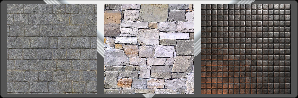
\includegraphics[scale=0.6]{images/01a_ui_texture.png}
  }
  \qquad
  \subfloat[\centering types]{
    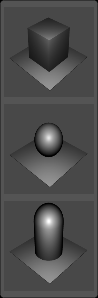
\includegraphics[scale=0.6]{images/01b_ui_type.png}
  }
  \caption{UI panels}
\end{figure}

The two panels are children of the same canvas, which itself is a child of a \textit{UI} object. This object is for organisational purposes and for housing the script component for handling UI interactions.

Each panel has 3 buttons, which display the appropriate provided texture. The type of these textures has to be changed to \textit{Sprite} in order to use them in the UI. The panels have a vertical/horizontal layout group component to evenly space the buttons within the panels. Anchor presets are used to align the panels to the middle left or centre bottom.

Each button has its \texttt{OnClick} handled by the script component in the \textit{UI} object mentioned earlier. The texture buttons use \texttt{UIManager.OnTextureClick} and the primitive type buttons use \texttt{UIManager.OnPrimitiveClick}. From the inspector, an argument is passed to these functions, which is an integer that corresponds to the enums \texttt{UIManager.Texture} and \texttt{PrimitiveType}, respectively.

Upon a button being clicked, the appropriate handler is called. It converts the integer argument to the corresponding enum and stores the enum in the public field \texttt{UIManager.texture} or \texttt{UIManager.primitive}.

\subsection{Primitive Creation}
When the user left clicks on the base or an existing primitive, a new primitive is created using the selected texture and primitive type. The new primitive can be placed at an arbitrary location on the base, or be aligned to the selected face of an existing primitive. A new primitive cannot be placed if it will collide with an existing primitive. There is a \texttt{CubeManager} object with a script component responsible for this.

\subsubsection{Position Calculation}
To determine the position of the new primitive, a ray is cast from the current mouse position. To avoid casting rays when the UI is being clicked, \texttt{EventSystem.IsPointerOver\-GameObject} is checked before casting the ray. When a ray hits something due to a left click, \texttt{CreatePrimitive} is called. It uses \texttt{GetNewPosition} to get the position for the new primitive based on the ray cast hit's information.

If the ray hit the base, then the position is half a unit up from the hit point so that the bottom face of the object is adjacent to the top face of the base. Otherwise, it hit an existing primitive, and the new position is the position of the hit object plus the normal of that object. The \textit{normal} is a unit vector perpendicular to the face the ray hit. This is what causes the object to be aligned to the face.

Because capsules are 2 units tall rather than 1 unit tall, and their origin is at the centre rather than at the bottom or top halves, half a unit is added to the $y$ component of the final position vector for capsules. This prevents the capsule from intersecting with the base or other primitives. It also causes the capsule's bottom half to align to an adjacent face rather than the capsule's centre aligning to that face.

\subsubsection{Alignment for Spheres and Capsules}
When aligning an object to a sphere or a capsule, it is aligned as if the hit object was a cube. This makes adjacent objects nicely align in a grid. To achieve this, spheres and capsules are given a child object which has a unit \texttt{BoxCollider} and is centred on the parent. Unity treats a collision with a child as a collision with the parent too. When a ray is cast, it collides with the face of the child \texttt{BoxCollider} rather than the round surface of the sphere or capsule.

Capsules are a special case since they're taller than 1 unit. While one \texttt{BoxCollider} with a height of 2 could be used, it would cause new primitives to be aligned with the middle of the capsule, which is out of alignment with the grid. Instead, the capsule uses two unit \texttt{BoxCollider}s: one for the lower half and a second for the upper half. Because the \texttt{RaycastHit.transform} returns the transform of the collider, \texttt{GetNewPosition} just thinks it's trying to align to a cube when a capsule is hit.

\begin{figure}[htp]
  \centering
  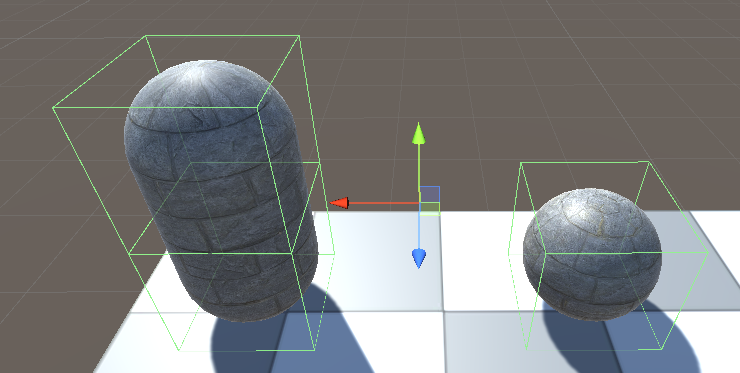
\includegraphics[width=\linewidth]{images/02_box_colliders.png}
  \caption{Rendered \texttt{BoxCollider}s}
\end{figure}

Regarding implementation details, each \texttt{BoxCollider} needs to be in a separate child, since an object cannot have more than one collider component of the same type. Furthermore, to position the colliders in the lower/upper halves, the transform of the child must be changed rather than the centre of the collider component. Otherwise, \texttt{RaycastHit.transform.position} is indistinguishable for the lower and upper halves.

\begin{figure}[htp]
  \centering
  \subfloat[\centering bottom half]{
    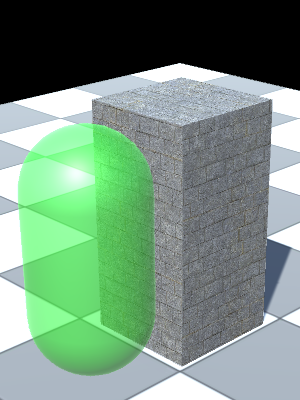
\includegraphics[width=0.28\linewidth]{images/03a_capsule_align_bottom_half.png}
  }
  \qquad
  \subfloat[\centering top half]{
    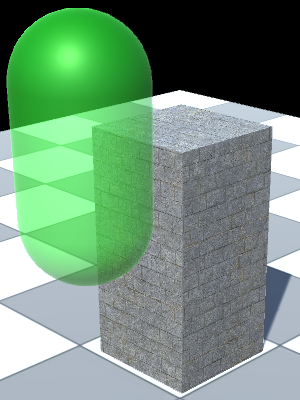
\includegraphics[width=0.28\linewidth]{images/03b_capsule_align_top_half.png}
  }
  \qquad
  \subfloat[\centering above]{
    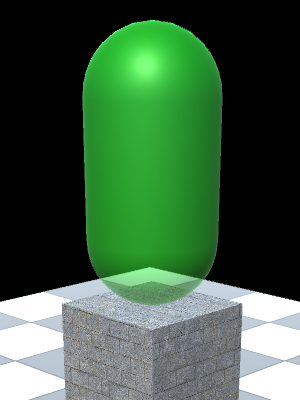
\includegraphics[width=0.28\linewidth]{images/03c_capsule_align_above.png}
  }
  \caption{Capsule alignment}
\end{figure}

\subsubsection{Placement Collision}
A primitive cannot be placed if it collides with an existing primitive. This collision always uses the regular colliders of the primitives rather than the \texttt{BoxCollider}s described previously. This is done by putting the primitives and the \texttt{BoxCollider} children in separate layers. When casting rays for collision detection, a layer mask is used to exclude all layers except for the primitives (the base is also excluded).

Collision checks are performed by \texttt{IsColliding} using \texttt{Physics.CheckSphere} if the new object will be a sphere, \texttt{Physics.CheckCapsule} if it's a capsule, and \texttt{Physics.CheckBox} for every other type. These functions are given dimensions such that the area checked for collision is equivalent to the size of the new object being created. However, because Unity considers adjacent faces to be colliding, \texttt{Physics.defaultContactOffset} is subtracted from the radius used with the collision check functions.

\subsubsection{Selected Texture and Type}
The public field \texttt{CubeManager.ui} is used to give the \texttt{CubeManager} access to the \texttt{UIManager} for its public \texttt{texture} and \texttt{primitive} fields. The \texttt{ui} field is set in the inspector.

Each available texture for the primitive has a corresponding material. The \texttt{CubeManager} is initialised by loading these three materials. It uses \texttt{Resources.Load}, so the materials have to be within the \textit{Assets/Resources/} directory. When the materials are loaded, they are stored in a dictionary which maps the materials to the corresponding \texttt{UIManager.Texture} enum value.

A primitive is created by passing \texttt{UIManager.primitive} to \texttt{GameObject.Create\-Primitive}. Next, the material is retrieved from the dictionary using \texttt{UIManager.texture} as the key. It is then set on the new object by assigning it to the \texttt{material} field of the object's \texttt{MeshRenderer} component.

\subsection{Placement Guide}
When the mouse is hovered over the base or a placed object, a visual guide for placement is shown. This guide has the same shape as the currently selected primitive type, but it's texture is simply a translucent colour. It's green if the placed object will align with an existing object, yellow if it doesn't align, and red if it collides with an existing object.

\begin{figure}[htp]
  \centering
  \subfloat[\centering aligned]{
    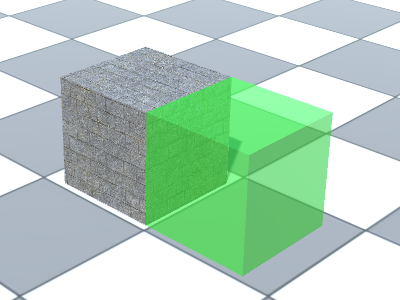
\includegraphics[width=0.28\linewidth]{images/04a_guide_green.png}
  }
  \qquad
  \subfloat[\centering non-aligned]{
    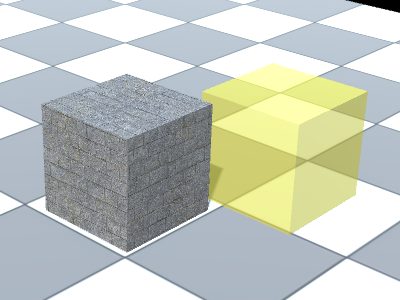
\includegraphics[width=0.28\linewidth]{images/04b_guide_yellow.png}
  }
  \qquad
  \subfloat[\centering colliding]{
    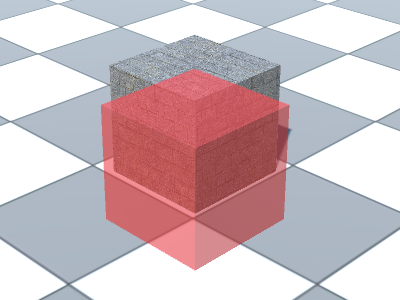
\includegraphics[width=0.28\linewidth]{images/04c_guide_red.png}
  }
  \caption{Placement guide}
\end{figure}

When a ray is cast, but neither the left nor the right mouse buttons were clicked, \texttt{ShowGuide} is called to display the visual guide. There \texttt{CubeManager} has three children, one for each primitive. The guide is shown by activating and deactivating these child primitives. These primitives are stored in a dictionary when the \texttt{CubeManager} is initialised. Furthermore, the \texttt{CubeManager} keeps track of the active object in a private field.

\texttt{ShowGuide} first gets the primitive from the dictionary using \texttt{UIManager.primitive} as a key. Next, it sets its position to what \texttt{GetNewPosition} returns. Then, it sets the colour for the primitive's material; if \texttt{IsColliding} is \texttt{true}, then the colour is set to red. Finally, it deactivates the active primitive, saves the new primitive as the active one, and then activates it.

The children are in layer 2, which is ignored by ray casts by default. This will ensure that the visual guide isn't position adjacent to the guide in the previous frame. The children also use a custom material, which is really just the default material but with a flag changed to support transparency. The actual transparency is set in the script by setting the alpha channel to 0.5 when the material's colour is changed.

\subsection{Primitive Destruction}
When a placed object is right-clicked, it is destroyed with an explosion effect. When a primitive is created, the provided \texttt{TriangleExplosion} script is attached as a component. To trigger it, the component is retrieved and its \texttt{SplitMesh} method is triggered using \texttt{StartCoroutine}. This allows the explosion effect to be spread across several frames.

\begin{figure}[htp]
  \centering
  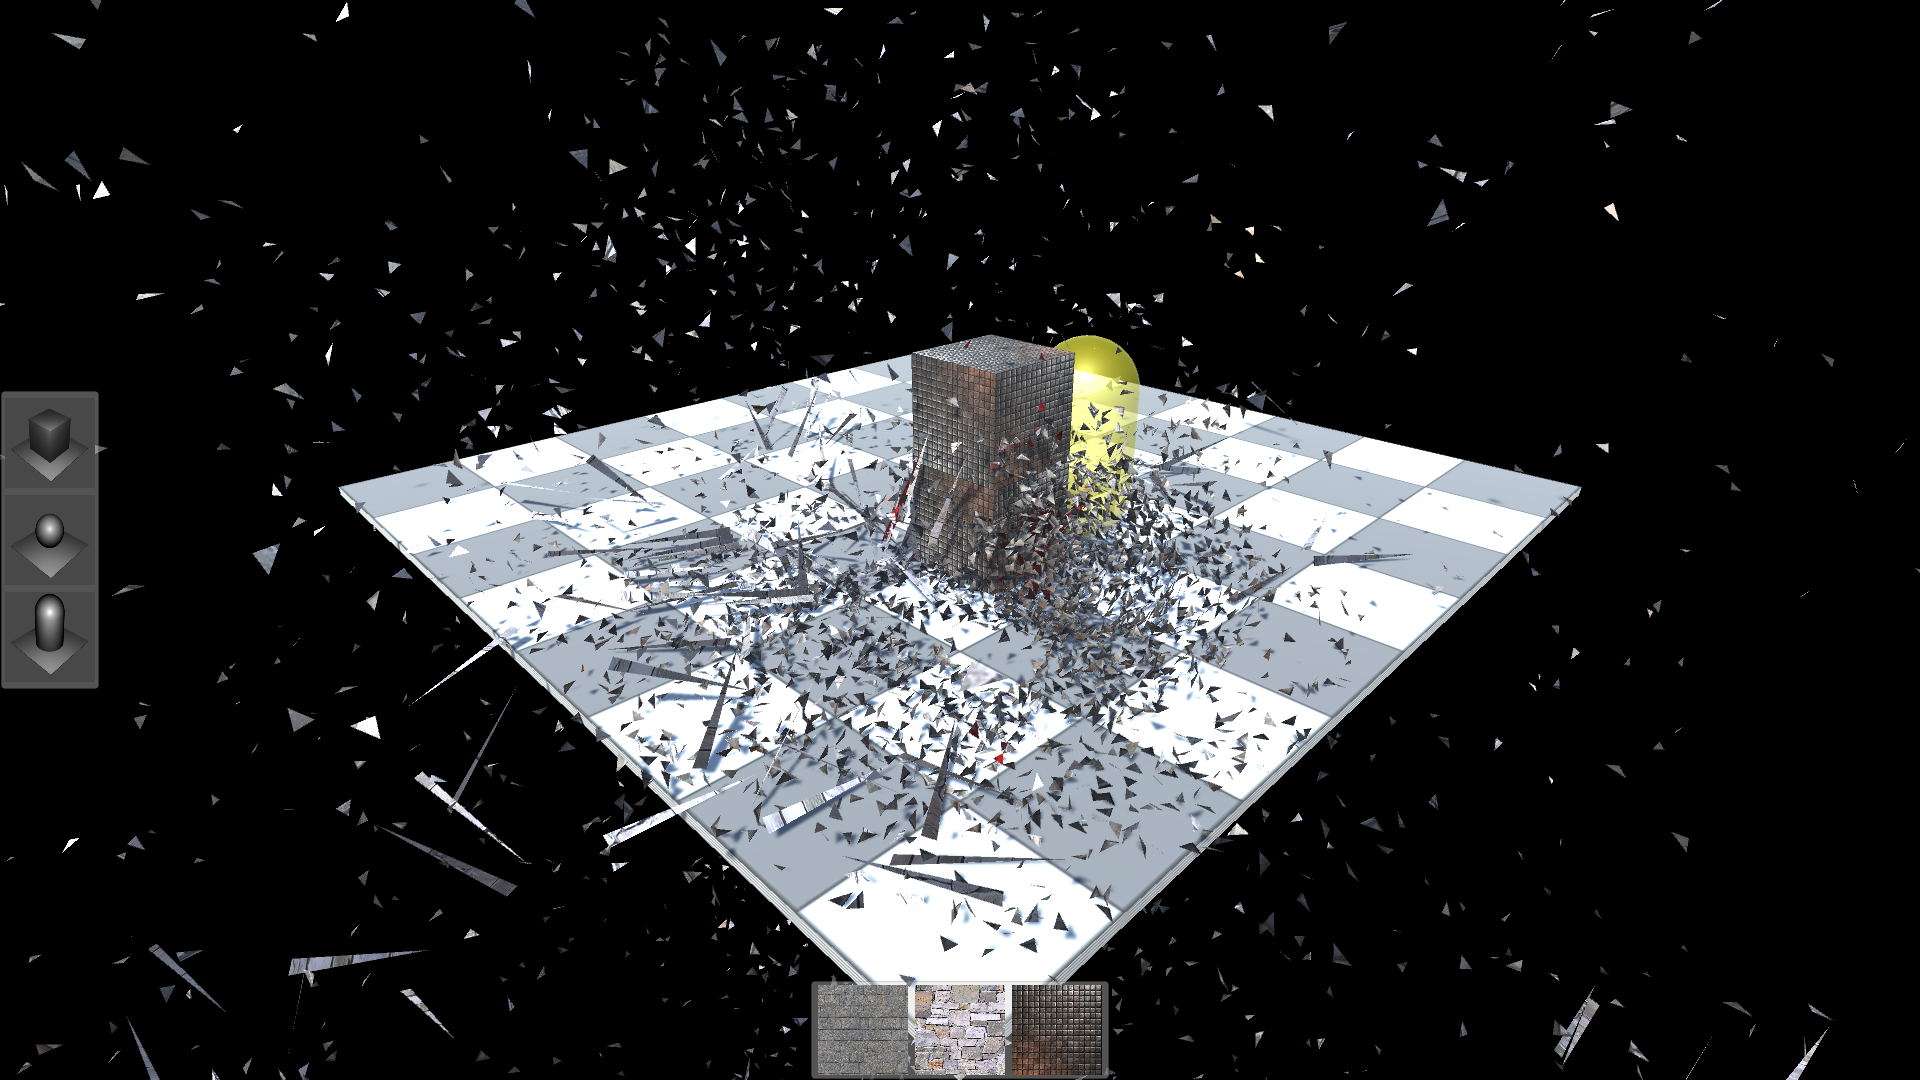
\includegraphics[width=\linewidth]{images/05_explosion.png}
  \caption{Explosions}
\end{figure}

The \texttt{TriangleExplosion} is modified to change the layer of the created triangles such that they are ignored by ray casts. This prevents issues like primitive creation aligning to the triangles.

The script component is retrieved using \texttt{GetComponentInParent}, which looks in either the current object or its parent. Recall that \texttt{RaycastHit.transform} returns the transform of the collider, which won't necessarily be the object that has the explosion script; spheres and capsules having children for colliders, which don't have the script component.

\section{Challenges}
It was challenging to figure out how to align to spheres and capsules as if they were cubes. It was especially difficult for capsules, since they need 2 collider children. A subtle error I made was to offset the colliders rather than offsetting their transforms, which caused a lot of confusion. The child collider approach was not even evident at first, so at first there was a lot of bespoke logic for handling position calculations for capsules (which didn't even work).

It was also unclear how to trigger the explosion script, but I eventually came across a tip to use \texttt{StartCoroutine}.

\section{Lessons Learned}
There were three big learning outcomes for me: general familiarisation with the Unity Editor, Unity's collision system, and Unity's UI system. I feel more comfortable with basic tasks like creating objects and using the inspector. I do not take this for granted since I struggled with it the first couple of days I used the Unity Editor. I learned about various collider components, compound colliders, and physics functions for checking collision. Finally, I learned how to make basic UI layouts with layout groups and anchors.

\end{document}
